\section{Paper-specific project}\label{sec:project}
In this section, we compare two of the data fission procedures introduced in \cite{leiner2022data} for Gaussian distributed data against data splitting, in the context of constructing selective CIs in fixed-design linear regression models. Suppose we are given a set of $n$ observations such that for $i\in\{1,\dots,n\}$, 
\[
y_i = x_i^\top \beta + \eps_i,
\]
where for some $p\in\nats$ and known $\sigma>0$, $x_i\in\reals^p$, $\eps_i\distiid \distNorm(0,\sigma^2)$, and $\beta\in\reals^p$. Equivalently, we can write $Y_i\distas\distNorm(x_i^\top\beta, \sigma^2)$. Note here we assume that the covariates $x_i$'s are fixed. The goal is to first perform variable selection and then construct CIs for the regression coefficients corresponding to the selected variables. We would like to compare variable selection accuracy as well as inference quality obtained using the following three procedures:
\begin{itemize}
\item Data fission (P1): for each $i\in\{1,\dots,n\}$, and some fixed $\tau\in(0,\infty)$, draw $Z_i\distas\distNorm(0,\sigma^2)$. Let $f_\tau(Y_i) = Y_i + \tau Z_i$, $g_\tau(Y_i) = Y_i - \tau^{-1}Z_i$. Then $f_\tau(Y_i)\indep g_\tau(Y_i)$ and $f_\tau(Y_i)\distas\distNorm(x_i^\top\beta, (1+\tau^2)\sigma^2)$, $g_\tau(Y_i)\distNorm(x_i^\top\beta, (1+\tau^{-2})\sigma^2)$. We use $(f_\tau(Y_i))_{i=1}^n$ for selection and $(g_\tau(Y_i))_{i=1}^n$ for inference.
\item Data fission (P2): for each $i\in\{1,\dots,n\}$, and some fixed $\tau\in(0,\infty)$, draw $Z_i\distas\distNorm(Y_i,\tau\sigma^2)$. Let $f_\tau(Y_i) = Z_i$, $g_\tau(Y_i) = Y_i$. Then $f_\tau(Y_i)\distas\distNorm(x_i^\top\beta, (1+\tau)\sigma^2)$, $g_\tau(Y_i)\given f_\tau(Y_i)\distas\distNorm\left(\frac{\tau}{\tau+1}x_i^\top\beta + \frac{1}{\tau+1}f_\tau(Y_i), \frac{\tau}{\tau+1}\sigma^2\right)$. We use $(f_\tau(Y_i))_{i=1}^n$ for selection and $(g_\tau(Y_i))_{i=1}^n$ for inference.
\item Data splitting: for some fixed $a\in\{\frac{1}{n}, \frac{2}{n}, \dots, 1\}$, randomly draw $an$ observations from $(Y_i)_{i=1}^n$ without replacement. Without loss of generality, denote the first $an$ observations as those that are selected. Use $(Y_i)_{i=1}^{an}$ for selection and $(Y_i)_{i=an+1}^n$ for inference.
\end{itemize}
We begin by observing the three datasets used for the selection step. Both data fission procedures inflate the variance of each observation without changing their underlying means. Data splitting, on the other hand, directly reduces the number of observations without perturbing their underlying distributions. This also introduces uncertainty to the selection step. It is then of interest to compare variable selection accuracies under different sample sizes and the amount of variance inflated. However, recall that from the Fisher information perspective, to make the comparison fair, we set $a = \frac{1}{1+\tau^2}$. If we fix the data splitting procedure to be partioning the original dataset into two subsets of equal sizes ($a=\frac{1}{2}$), the comparison reduces to be about varying the sample sizes.

We now consider the inference stage. Suppose that the selected model is $M\subset\{1,\dots,p\}$ and that
\[
X_M = \begin{bmatrix} x_{M,1}, \dots, x_{M,n} \end{bmatrix}^\top, \quad Y = \begin{bmatrix} Y_1, \dots, Y_n \end{bmatrix}^\top,
\]
where $x_{M,i}$ is a vector consisting of only the covariates corresponding to the selected features. We then have our ideal target parameter given $M$ as
\[
\beta^\star(M) = \argmin_{\tilde{\beta}} \EE_Y \|Y - X_M\tilde{\beta}\|^2 = (X_M^\top X_M)^{-1}(X_M^\top\mu)
\]
where $\mu = \begin{bmatrix} x_1^\top\beta, \dots, x_n^\top\beta \end{bmatrix}^\top$. However, since we are using slightly perturbed datasets for inference, our estimator $\hbeta(M)$ given the model $M$ for each of the three procedures are
\begin{itemize}
\item Data fission (P1): $\hbeta(M) = (X_M^\top X_M)^{-1}X_M^\top g_\tau(Y) \distas \distNorm(\beta^\star(M), \sigma^2(1+\tau^{-2})(X_M^\top X_M)^{-1})$;
\item Data fission (P2):\\ $\hbeta(M) = (X_M^\top X_M)^{-1}X_M^\top g_\tau(Y) \given f_\tau(Y) \distas \distNorm(\frac{\tau}{\tau+1}\beta^\star(M) + \frac{1}{\tau+1}(X_M^\top X_M)^{-1}X_M^\top f_\tau(Y), \sigma^2\frac{\tau}{\tau+1}(X_M^\top X_M)^{-1})$;
\item Data splitting: $\hbeta(M) = (X_M^\top X_M)^{-1}X_M^\top Y \distas \distNorm(\beta^\star(M), \sigma^2(X_M^\top X_M)^{-1})$.
\end{itemize}
Note that here $f_\tau$ and $g_\tau$ are applied to each entry of $Y$ and that $X_M$ and $Y$ in data splitting only contains a subset set of $na$ observations.

Looking at the means of each estimator above, both the data fission (P1) and data splitting procedures target $\beta^\star(M)$. On the other hand, the mean of the data fission (P2) estimator depends on the realized values of the external random variable $Z$. Since $\EE[f_\tau(Y)] = \mu$, if we marginalize $f_\tau(Y)$ over the distribution of $\hbeta(M)$, data fission (P2) would also target the ideal parameter $\beta^\star(M)$. However, it is reasonable to suspect that this randomness might affect the quality of inference.

We now look at the variances of the three estimators. Similar to the selection stage, data fission (P1) inflates the variance of $\hbeta(M)$ by a function of $\tau$, and data splitting introduces additional uncertainty by reducing the sample size. However, in data fission (P2), the variance is deflated. Now suppose for each $i$, $x_i \distiid \pi$, for some distribution $\pi$, and assume that for all selected model $M$, $\EE[x_{M,1}x_{M,1}^\top]$ is finite and strictly positive. Then we have
\[
\frac{1}{n}X_M^\top X_M \convp \EE[x_{M,1}x_{M,1}^\top] \implies \left(\frac{1}{n}X_M^\top X_M\right)^{-1} \convp \left( \EE[x_{M,1}x_{M,1}^\top] \right)^{-1} \implies \left(X_M^\top X_M\right)^{-1} \convp \frac{1}{n}\left( \EE[x_{M,1}x_{M,1}^\top] \right)^{-1}.
\]
Under this assumption, the difference in inference between data splitting and data fission once again comes down to the sample size and the amount of variance inflated or deflated by $\tau$. We therefore set up our simulations as following. Note that this is mostly in line with Section 4 of \cite{leiner2022data}.

We set $a = \frac{1}{2}$ and $\tau=1$ to ensure the amount of Fisher information allocated to the selection stage is the same across all three methods. Let $p=20, \beta_1=\beta_{19}=1$, $\beta_2=\beta_{20}=-1$, and the rest of the entries in $\beta$ be $0$. The covariates are generated from the standard multivariate Guassian distribution. Note that there is no intercept term in our regression model. We then conduct selective inference with varying sample sizes $10, 20, 50, 100$ to evaluate how both the variable selection and inference performances across all three methods change under different sample sizes. To compare variable selection accuracy, we use as our metrics
\[
\text{power} = \frac{|j\in M: \beta_j \neq 0|}{|j\in [p]: \beta_j \neq 0|}, \quad \text{precision} = \frac{|j\in M: \beta_j \neq 0|}{|M|}.
\]
To compare the quality of inference, we use false coverage rate (FCR), avg. CI length, and avg. L2 error:
\[
\text{FCR} = \frac{|k\in M: [\beta^\star(M)]_k \notin CI_k|}{\max\{|M|, 1\}}, \quad \overline{\text{CI len.}} = \frac{\sum_{k\in M} |\text{CI}_k(2) - \text{CI}_k(1)|}{|M|}, \quad \text{L2 err.} = \frac{\| \beta^\star(M) - \hbeta(M) \|_2^2}{|M|}.
\]
To perform variable selection, we run LASSO using the \texttt{glmnet} package in \texttt{R} with the default settings and the regularization parameter set to \texttt{lambda.1se}. We repeat the above experiments $200$ times and report the median of the above metrics (excluding runs that do not end up selecting any variable in the selection step) in \cref{fig:median}. The same set of plots with the IQR of each metric, along with other details of the experiment is included in \cref{apdx:plots}. Note that since the IQRs have a lot of overlaps, the discussion below is only concerned with the average performance rather than individual trials. The code used to run the simulations and generate the plots can be found at \url{https://github.com/NaitongChen/QP-3}.

\captionsetup[subfigure]{labelformat=empty}
\begin{figure}[ht!]
\centering
\begin{subfigure}[b]{.32\columnwidth} 
    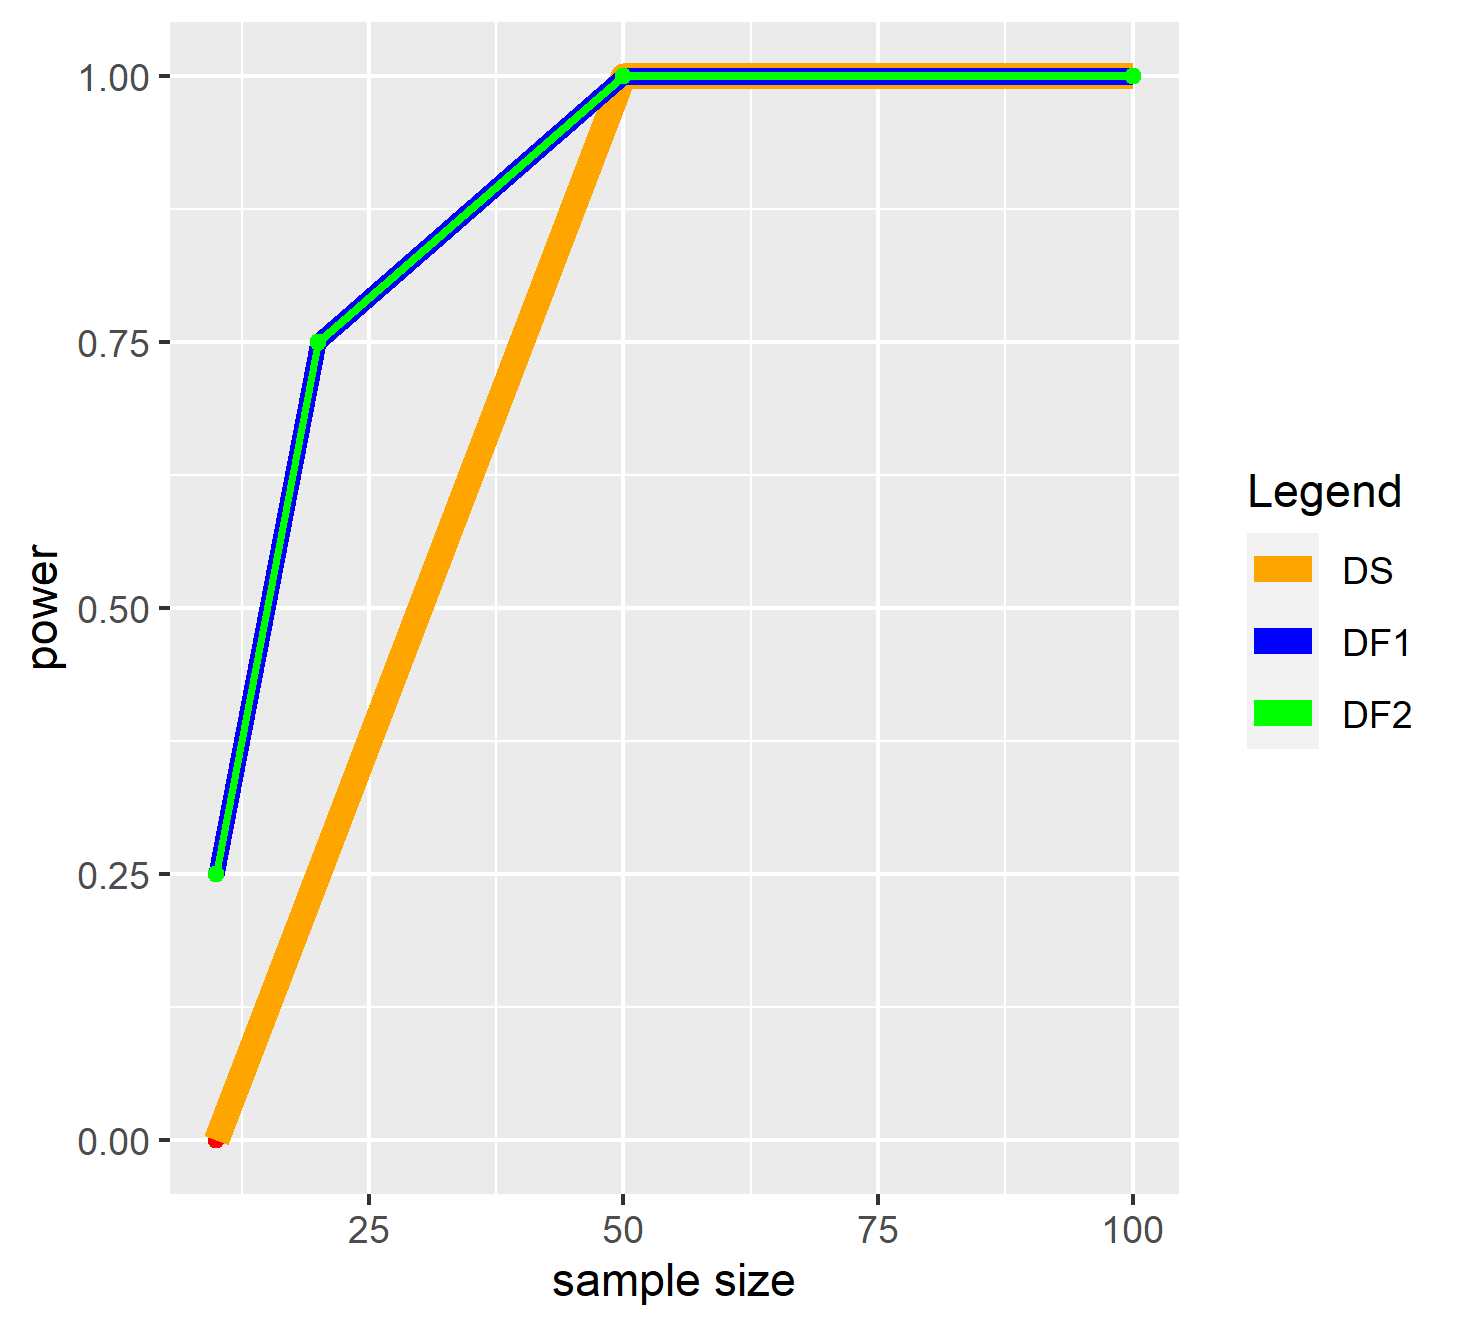
\includegraphics[width=\columnwidth]{../../plot/power_1.png}
    \caption{(a) Power}
    \label{fig:power}
\end{subfigure}
\hfill
\centering
\begin{subfigure}[b]{.32\columnwidth} 
    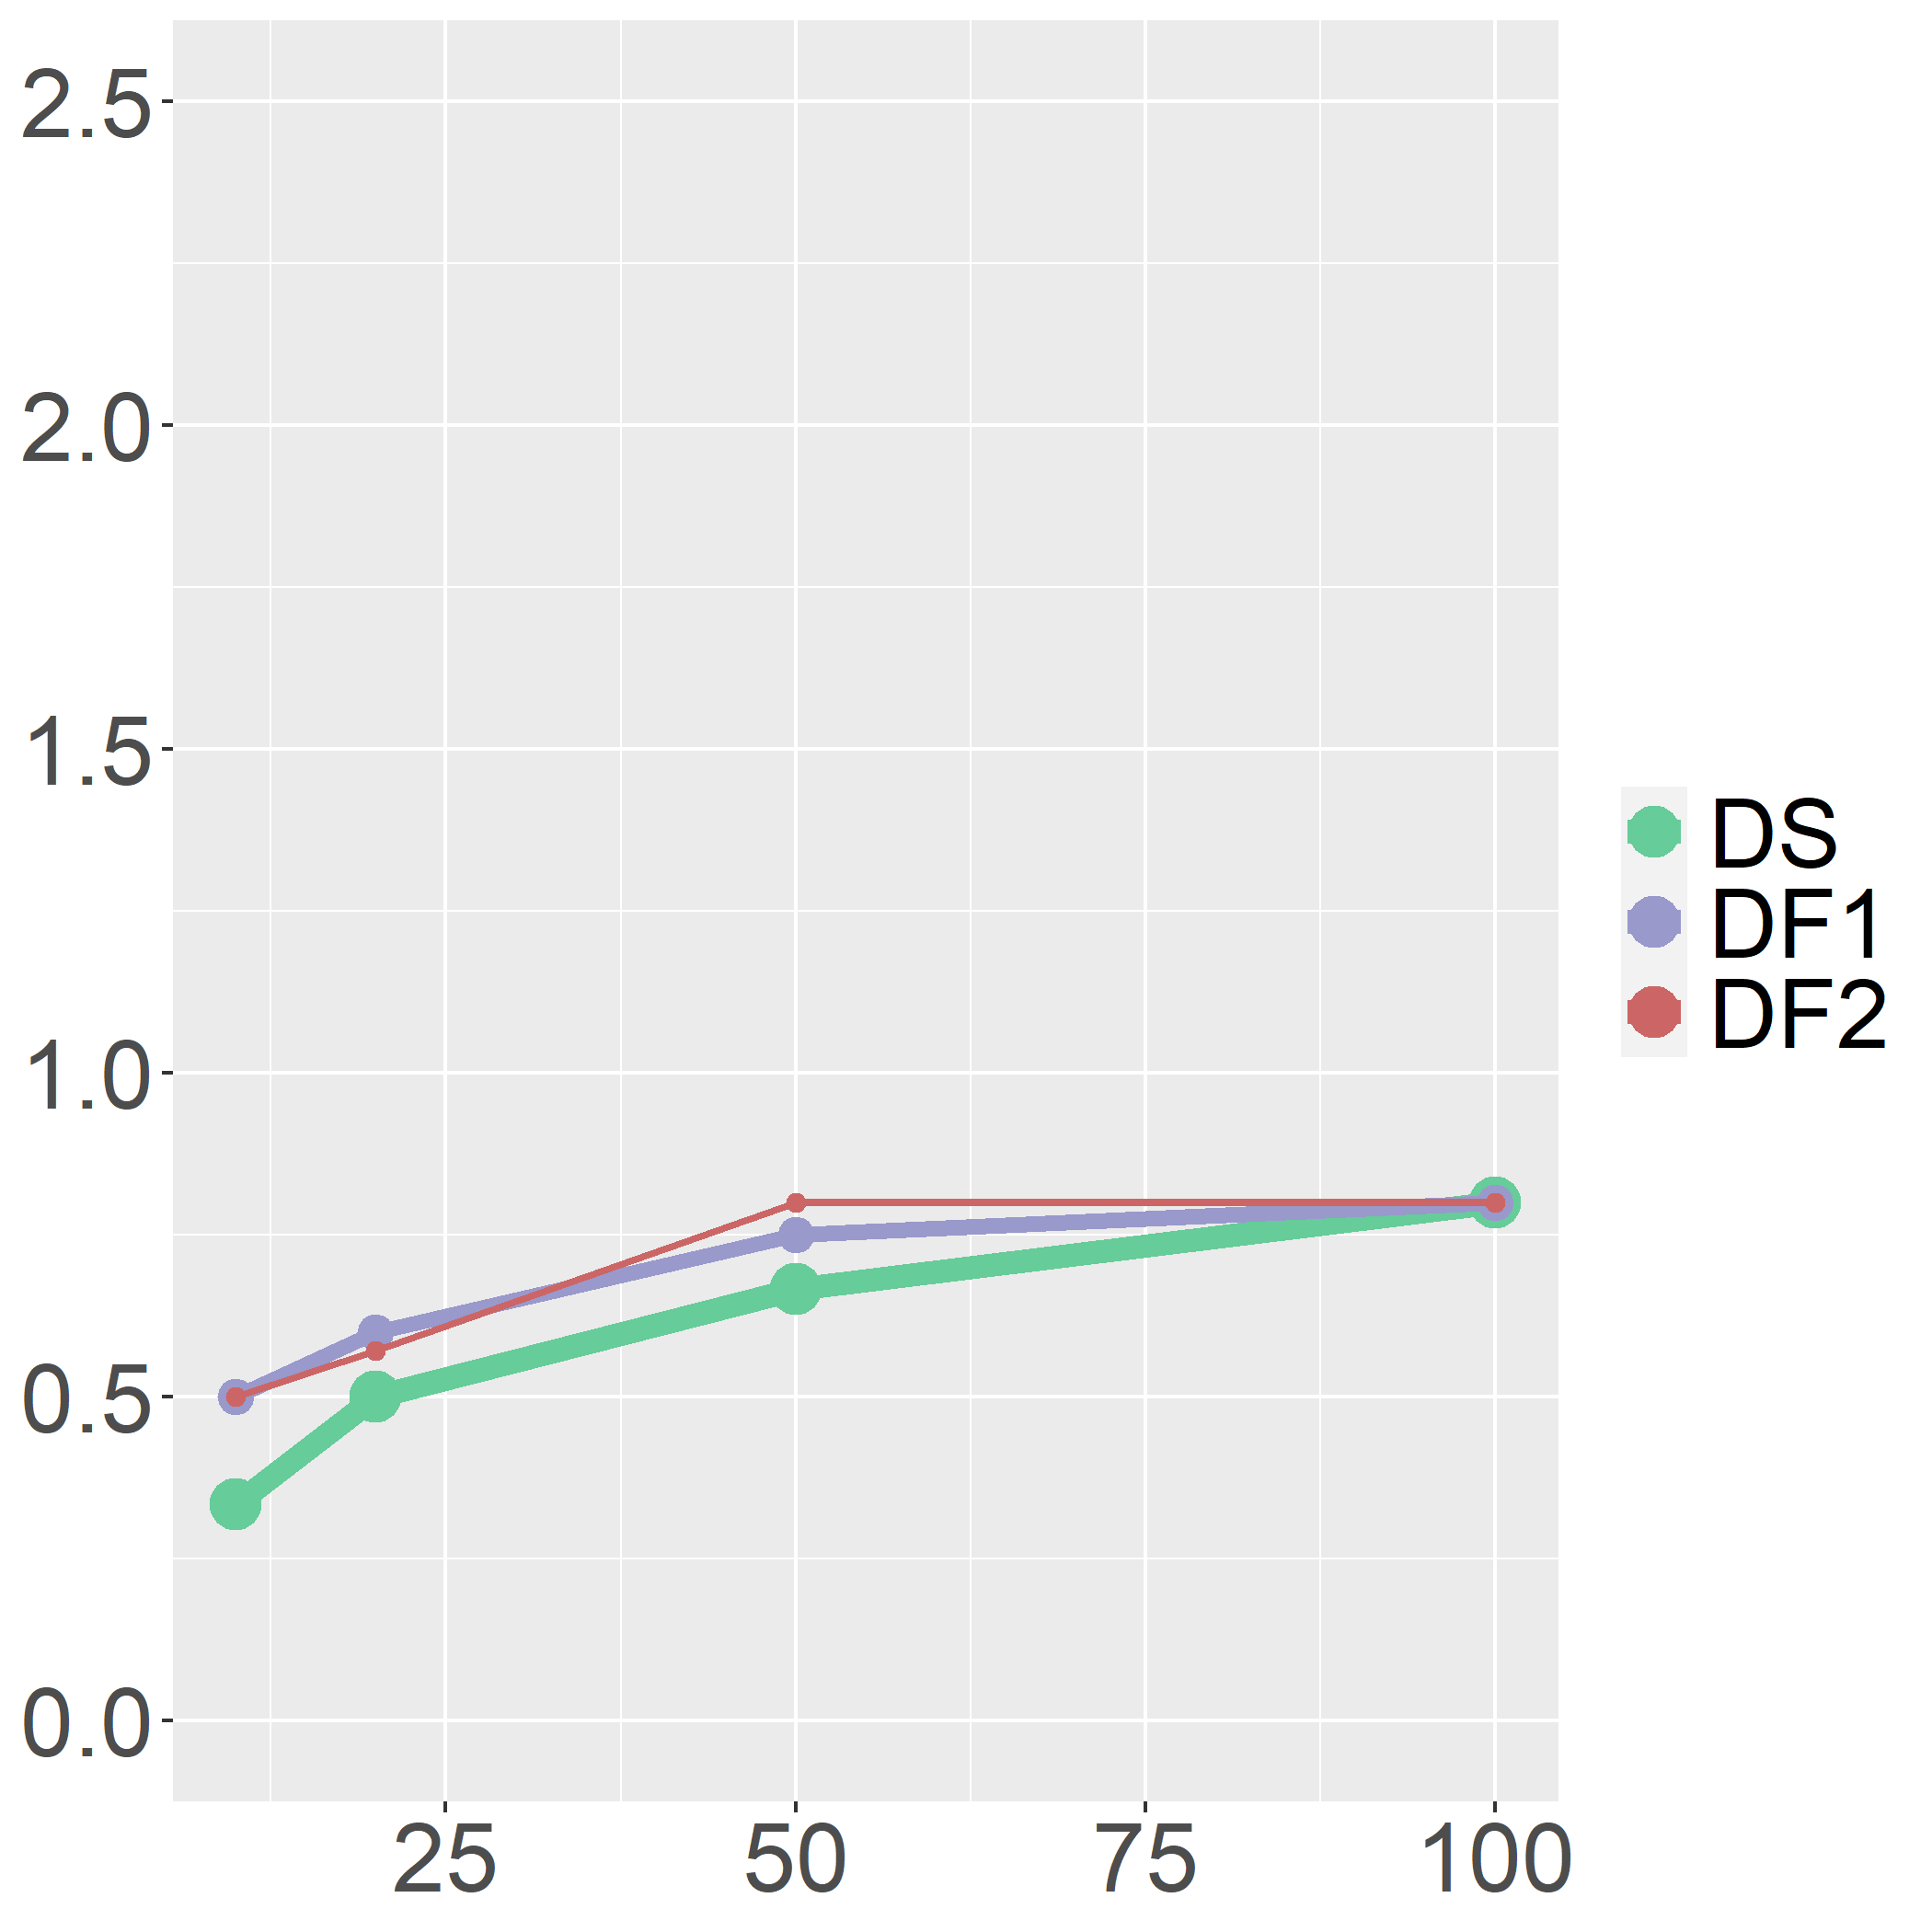
\includegraphics[width=\columnwidth]{../../plot/precision_1.png}
    \caption{(b) Precision}
    \label{fig:precision}
\end{subfigure}
\\
\centering
\begin{subfigure}[b]{.32\columnwidth} 
    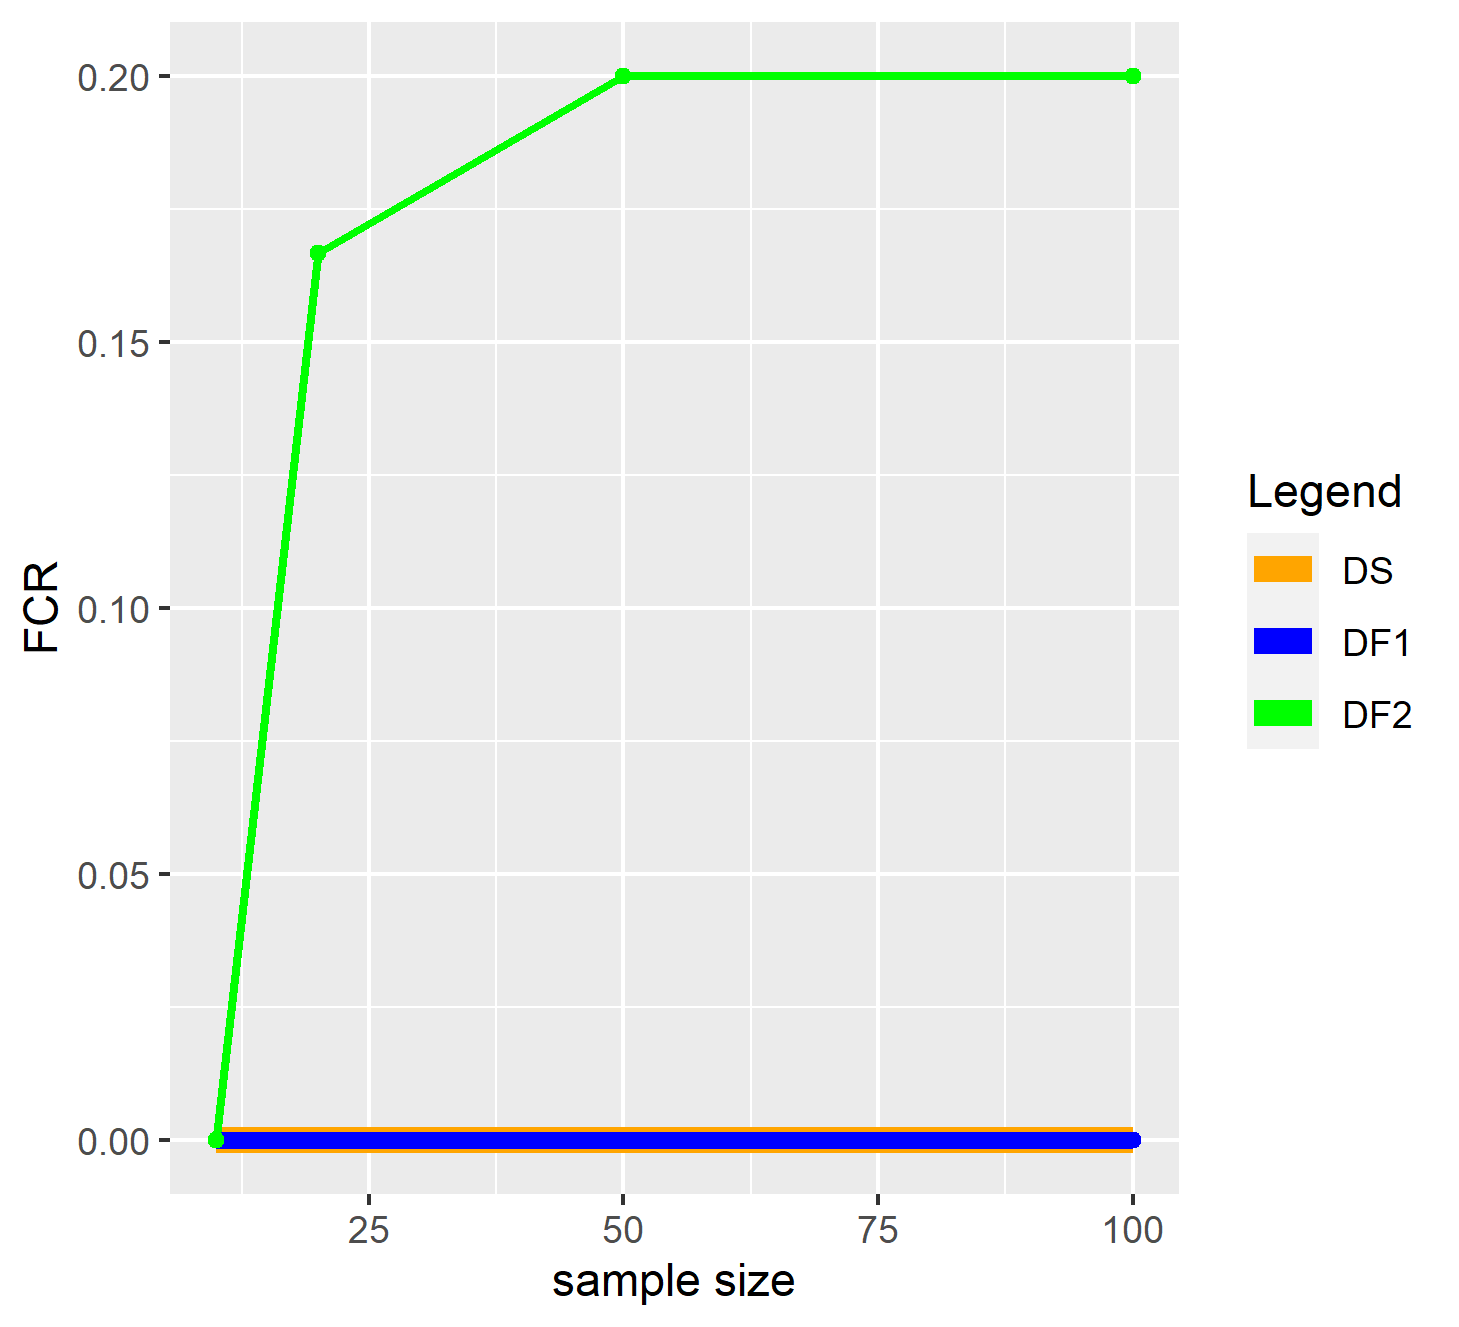
\includegraphics[width=\columnwidth]{../../plot/FCR_1.png}
    \caption{(c) FCR}
    \label{fig:fcr}
\end{subfigure}
\hfill
\centering
\begin{subfigure}[b]{.32\columnwidth} 
    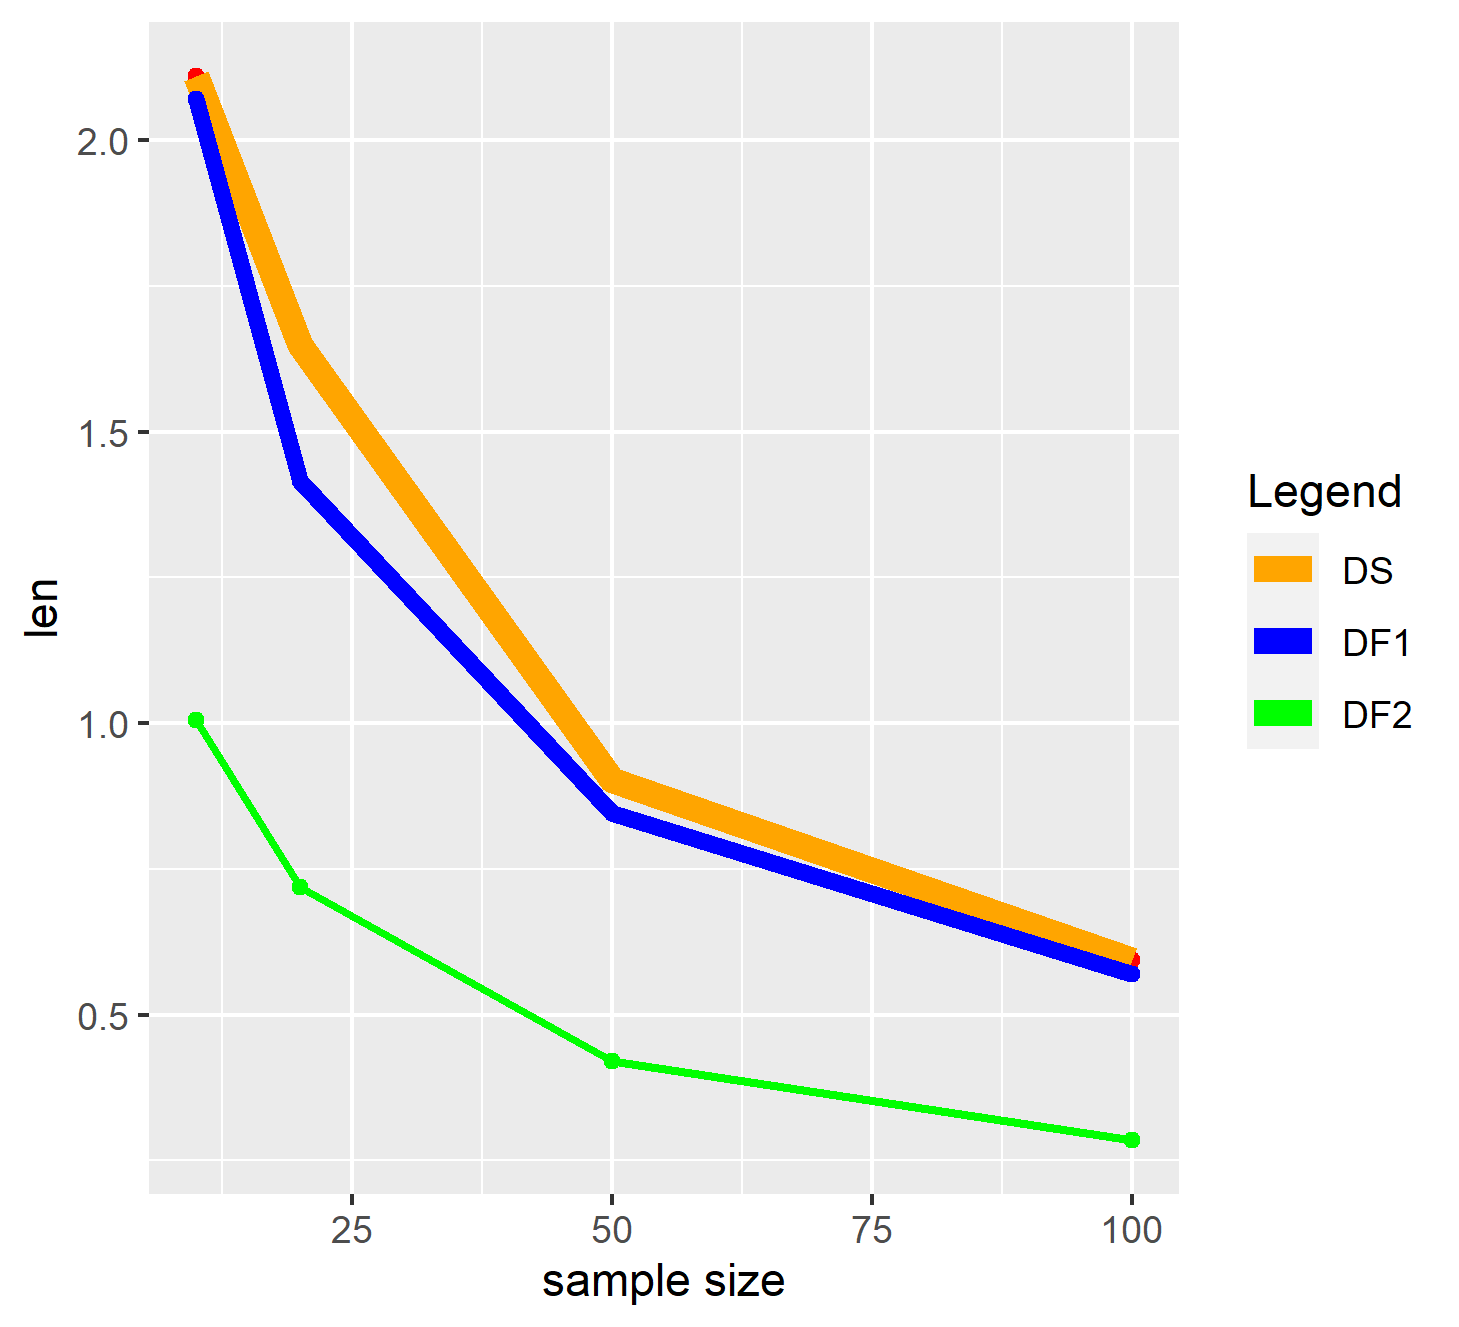
\includegraphics[width=\columnwidth]{../../plot/len_1.png}
    \caption{(d) Average CI length}
    \label{fig:ci}
\end{subfigure}
\hfill
\centering
\begin{subfigure}[b]{.32\columnwidth} 
    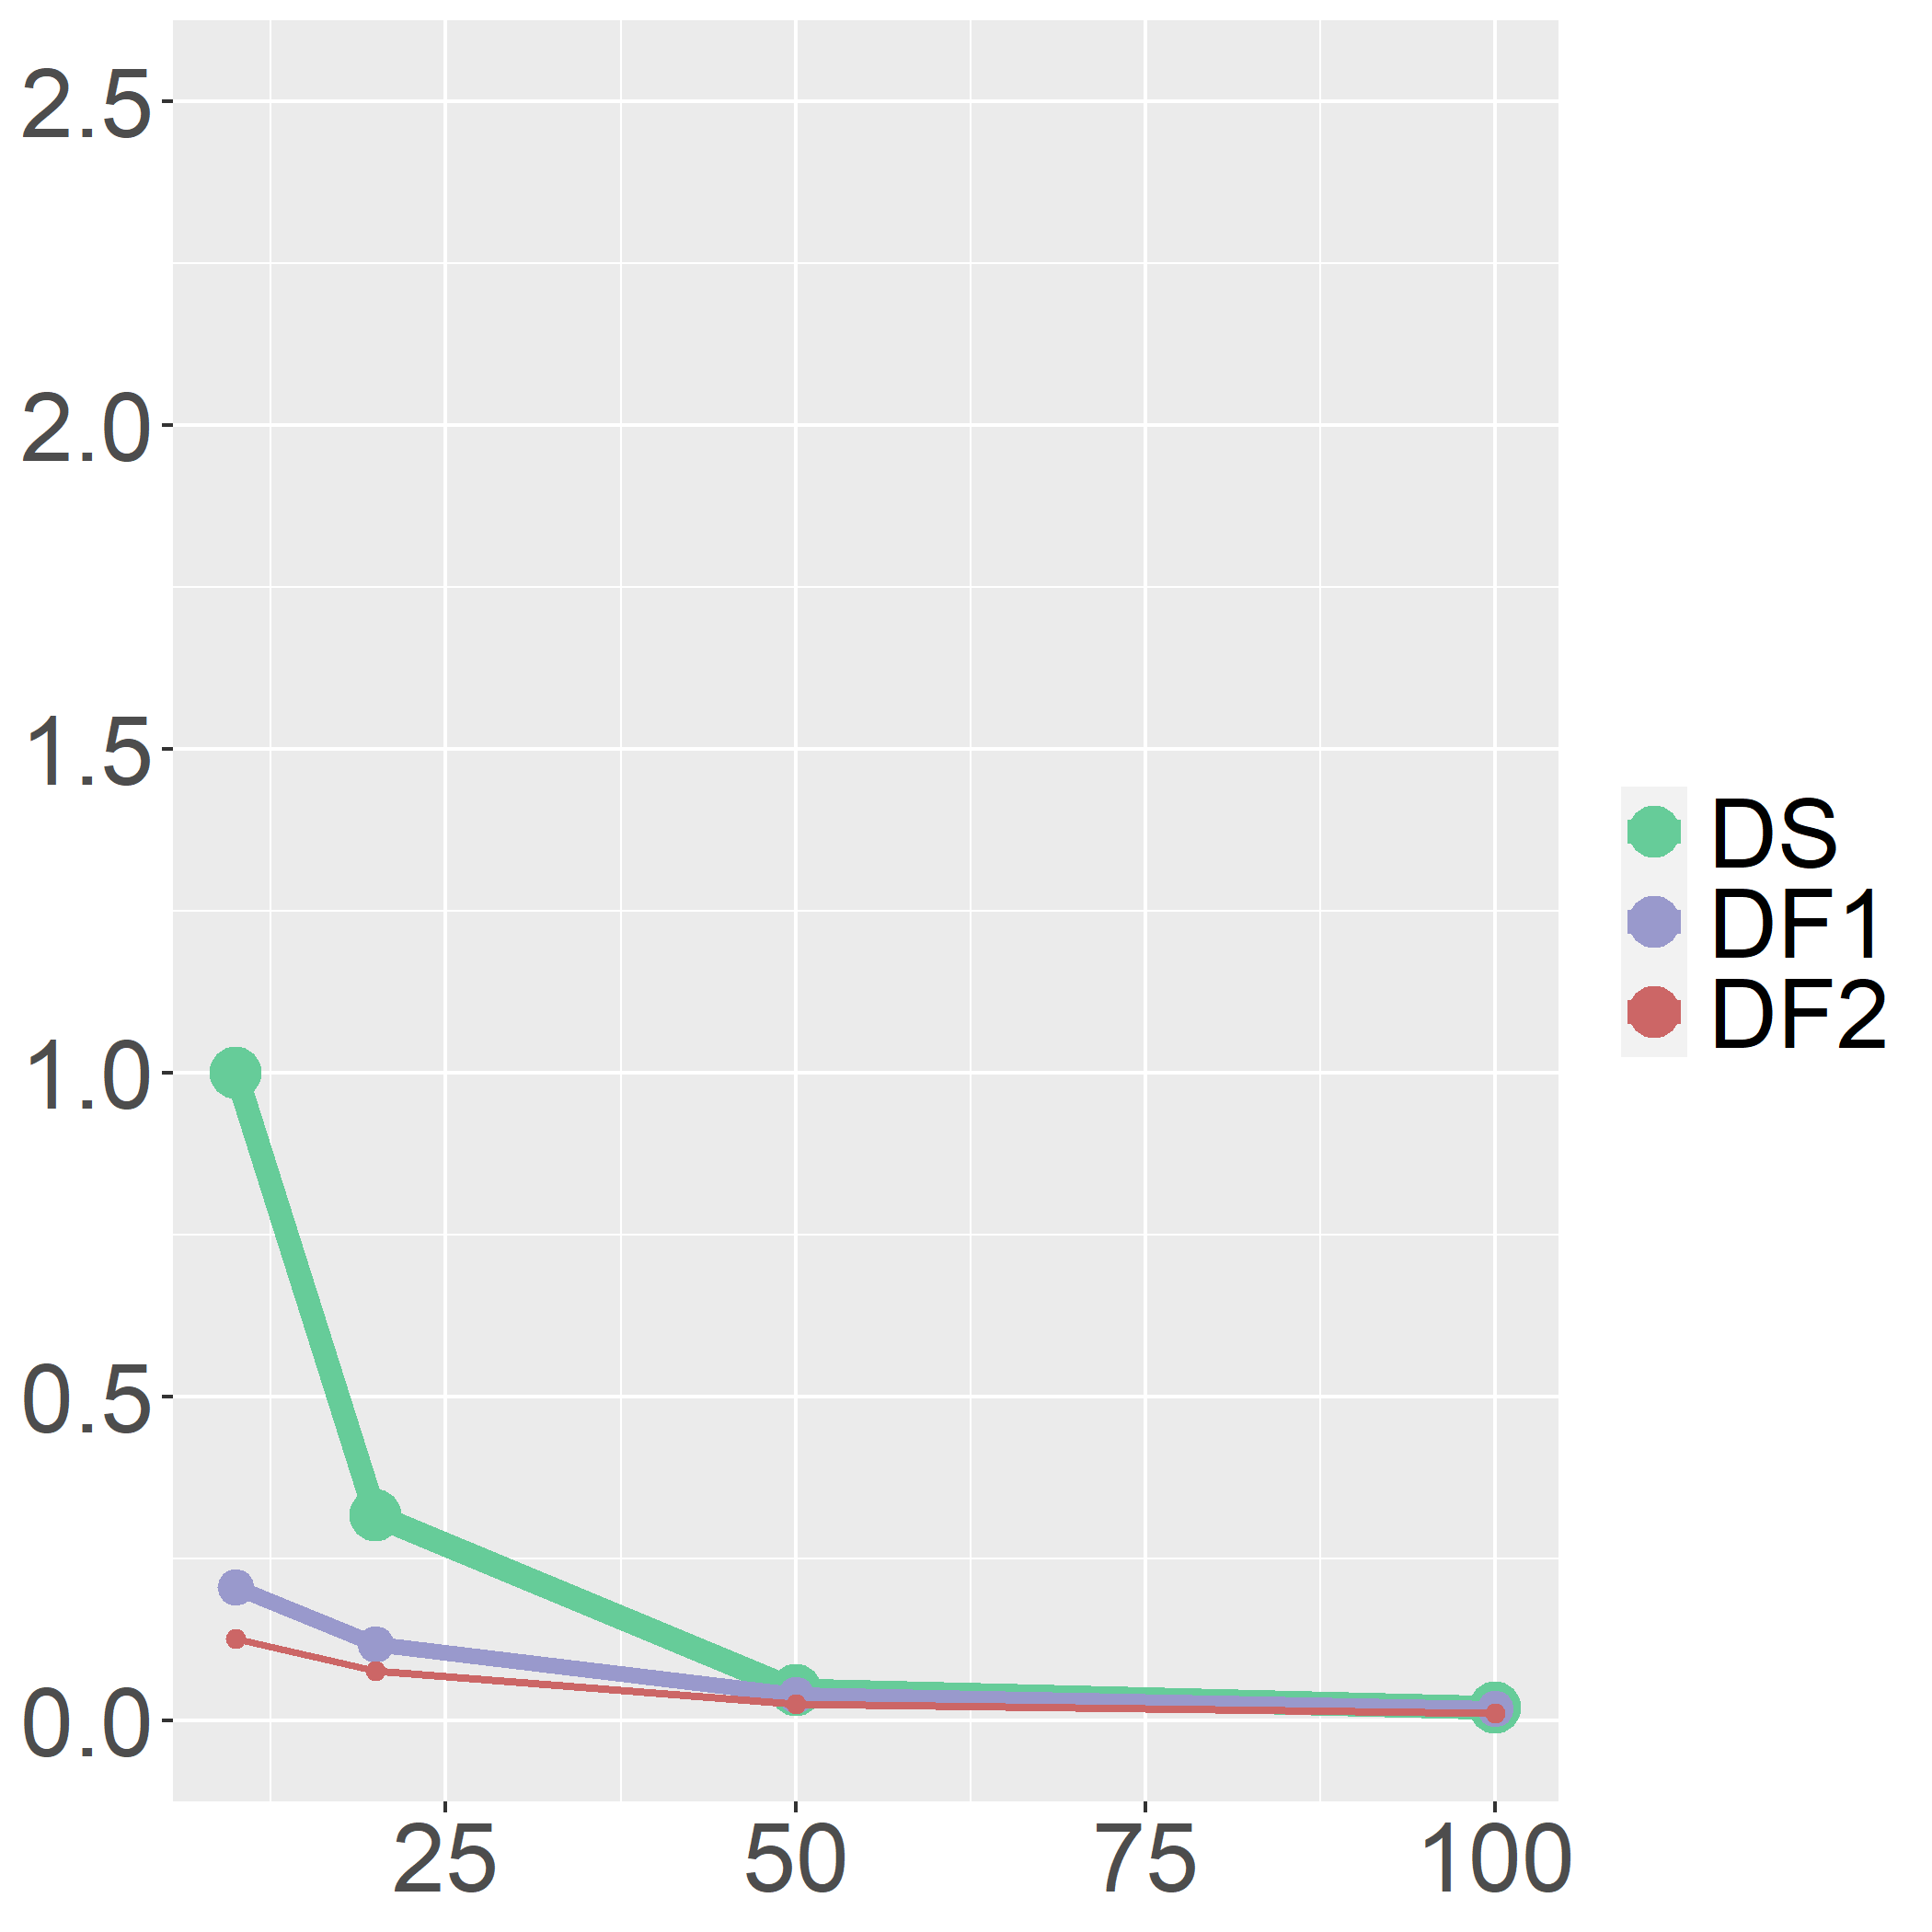
\includegraphics[width=\columnwidth]{../../plot/L2_1.png}
    \caption{(e) L2 error}
    \label{fig:l2}
\end{subfigure}
\hfill
\caption{Median of each metric across $200$ runs. The x-axis shows sample size, and the y-axis shows the value of each metric. DS refers to data splitting, DF1 and DF2 refer to data fission (P1) and data fission (P2).}
\label{fig:median}
\end{figure}

\subsection{Discussion of simulation results}

We begin by comparing variable selection accuracy through power and precision (\cref{fig:power,fig:precision}). Both metrics are similar across different sample sizes between the two data fission procedures, because they have the same $f_\tau(Y)$ marginal distributions with $\tau=1$. Compared to data splitting, data fission achieves higher power and precision, particularly when the sample size is small. When there are few observations, the disadvantage of data splitting working with only half of the observations becomes apparent. In particular, if we look at individual trials (\cref{fig:split10}), data splitting tends to miss true features and pick instead many false features, leading to suboptimal power and precision. This is to be expected, as when there is not a lot of information from the data, halving the number of observations would likely hinder the quality of variable selection. Although data fission inflates the variance of the observations by a factor of two, this seems to be a worthy price to pay in order to not reduce the number of observations used in the selection stage. As we increase the sample size, however, even half of the information becomes sufficient for variable selection, which makes the advantage of data fission less obvious.

We now look at the quality of inference through FCR, avg. CI length, as well as the L2 error between the estimated parameter and the ideal target of inference averaged by the number of variables selected. \cref{fig:fcr} shows that the median FCR for data splitting and data fission (P1) are both well below the target level $\alpha = 0.05$ using standard unadjusted $95\%$ CIs. Note that no correction is needed here since the proportion of CIs covering their respective parameters is expected to be $0.95$ \citep{benjamini2005false}. On the other hand, data fission (P2) has a much higher FCR (above the target level). This is due to the mean of $\hbeta(M)$ being different than $\beta^\star(M)$ and its variance being further deflated by the fission procedure. This is evident in \cref{fig:p2_100}. Interestingly, when the sample size is small ($n=10$), data fission (P2) is also able to control the FCR. One possible explanation is that the small sample size makes $(X^\top X)^{-1}$ highly variable and thus more likely widens the corresponding CI compared to when the sample size is large. It is also worth noting that having a low FCR does not necessarily mean that we recover the true parameters, because there is a discrepancy between $\beta$ and $\beta^\star(M)$, especially when the sample size is small (see for example \cref{fig:split10}).

In terms of the average length of $95\%$ CIs (\cref{fig:ci}), we see that data fission (P1) and data splitting are similar across all sample sizes. This suggests that the effect on the average length of CI is similar between inflating the variance by a factor of two and halving the number of observations. On the other hand, the average CI length for data fission (P2) is much smaller than the other two methods. This can be explained by the variance of $\hbeta(M)$ being deflated by the fission procedure and that there is no reduction in sample size.

Finally, we compare the L2 error between the estimated parameter and the ideal target of inference averaged by the number of variables selected in \cref{fig:l2}. We see here that, as expected, the L2 error decays as the sample size increases for all three methods. We see that the L2 error for data splitting is much higher than the two data fission procedures, particularly when the sample size is small. This is again due to data splitting reducing the sample size at the inference stage, which introduces uncertainty. It is somewhat surprising, however, to see that both data fission methods result in very similar L2 errors, despite data fission (P2) not targeting the ideal parameter ($\EE[\hbeta(M)] \neq \beta^\star(M)$). Considering the high FCR of data fission (P2), this implies that the effect of the discrepancy between $\EE[\hbeta(M)]$ and $\beta^\star(M)$ does not hinder the inference performance as much as the deflation of $\hbeta(M)$'s variance. This calls for further investigation, and a possible way to explore this issue is to compare the L2 errors across different $\sigma^2$ values in order to amplify the effect.